\documentclass[11pt]{article}
\usepackage{fullpage}
\usepackage{graphicx}
\usepackage{url}


\setlength{\parindent}{0pt}
\setlength{\parskip}{8pt}

\title{CS140 - Assignment 9\\\small{Due: Sunday, April 7th at 11:59pm}}
\author{}
\date{}


\begin{document}

\maketitle

\begin{center}
% \includegraphics[scale=0.6]{figures/magic_tree_2x.png}

\footnotesize{\url{https://xkcd.com/1569/}}
\end{center}


Note:  If not specified in the problem, you may assume whatever graph representation makes your algorithm more efficient (adjacency list or adjacency matrix).  State which one you are using.

\begin{enumerate}

\item \textbf{[10 points]} Induction on Trees

Use induction to prove that the number of degree-2 nodes in a non-empty binary tree is $1$ less than the number of leaves. Recall that the degree of a vertex in a tree is the number of children that it has.

\textbf{Answer}:

We want to show that the number of degree-2 nodes in a non-empty binary tree is $1$ less than the number of leaves. We choose to perform structural induction on the height of the binary tree to prove this.

For the base case, we realize that the smallest binary tree we could have is that which has a height of 0 ($h=0$). In that case, the binary tree is a single node, with no children, that is, a leaf. The number of degree-2 nodes in this case is 0 while the number of leaves is 1. Indeed, the number of degree-2 nodes in a non-empty binary tree is $1$ less than the number of leaves for the base case and so, the base case holds true.

For the inductive case (using structural induction), we assume that the statement we want to prove is true for the left and right subtrees (both binary trees, still) up to a height of $k$, where $k \le h$, where $h$ is the typical total height of the tree.

The inductive step to prove: We want to show that the number of degree-2 nodes in a non-empty binary tree is $1$ less than the number of leaves for a tree with a height of $k+1$.

The are 2 cases to consider:
\begin{enumerate}
    \item Where the root node is not a degree-2 node, that is, the root node has either only a left child (which goes on to form the entirety of the left subtree) or only a right child (which goes on to form the entirety of the right subtree). (Recall that we assume the statement holds for both the left and right subtrees).
    \item Where the root node is a degree-2 node, with both a left and right subtrees.
\end{enumerate}

Let us consider case 1, where we'll take it that the root node only has a left child. The number of degree-2 nodes in that case is the number of degree-2 nodes solely in the left subtree. The number of leaves for case 1 is also solely contributed by the number of leaves in the left subtree. But recall that our inductive hypothesis holds for either the left or right subtrees (in our case, the left one) and so for this case, we have shown that the number of degree-2 nodes in a non-empty binary tree is $1$ less than the number of leaves by the inductive hypothesis.

Let us next consider case 2. The number of degree-2 nodes is partly contributed by both the left and right subtrees, let's call them $l_2$ and $r_2$ respectively. Moreover, the root node (which makes the height of this tree $k+1$) is also a degree-2 node, so the total number of degree-2 nodes is $l_2+r_2+1$. The number of leaves is contributed solely by the left and right subtrees, which we can denote as $L(\#l)$ and $R(\#r)$ respectively. The total number of leaves, therefore, is $L(\#l)+R(\#r)$. Since the inductive hypothesis holds for both the left and right subtrees, the number of leaves, can be generalized to $(l_2+1)+(r_2+1)=l_2+r_2+1$ which is one more than the number of degree-2 nodes and so the inductive steps holds true.

We have shown the statement holds true via the base case and inductive step and can thus conclude that the number of degree-2 nodes in a non-empty binary tree is $1$ less than the number of leaves.

% ---- QUESTION 2 ----
\item \textbf{[5 points]} Someone suggests to you the following algorithm for finding the shortest path from node $s$ to node $t$ in a directed graph with some negative edges:  add a large constant to each edge weight so that all the weights become positive, then run Dijkstra's algorithm starting at node $s$, and return the shorted path found to node $t$.

Is this a valid method? Argue that it works correctly or give a counterexample.

\textbf{Answer}:

This is not a valid method for all cases of a directed graph with some negative edges. Here is our counterexample:

\begin{figure}[h]
\centering
    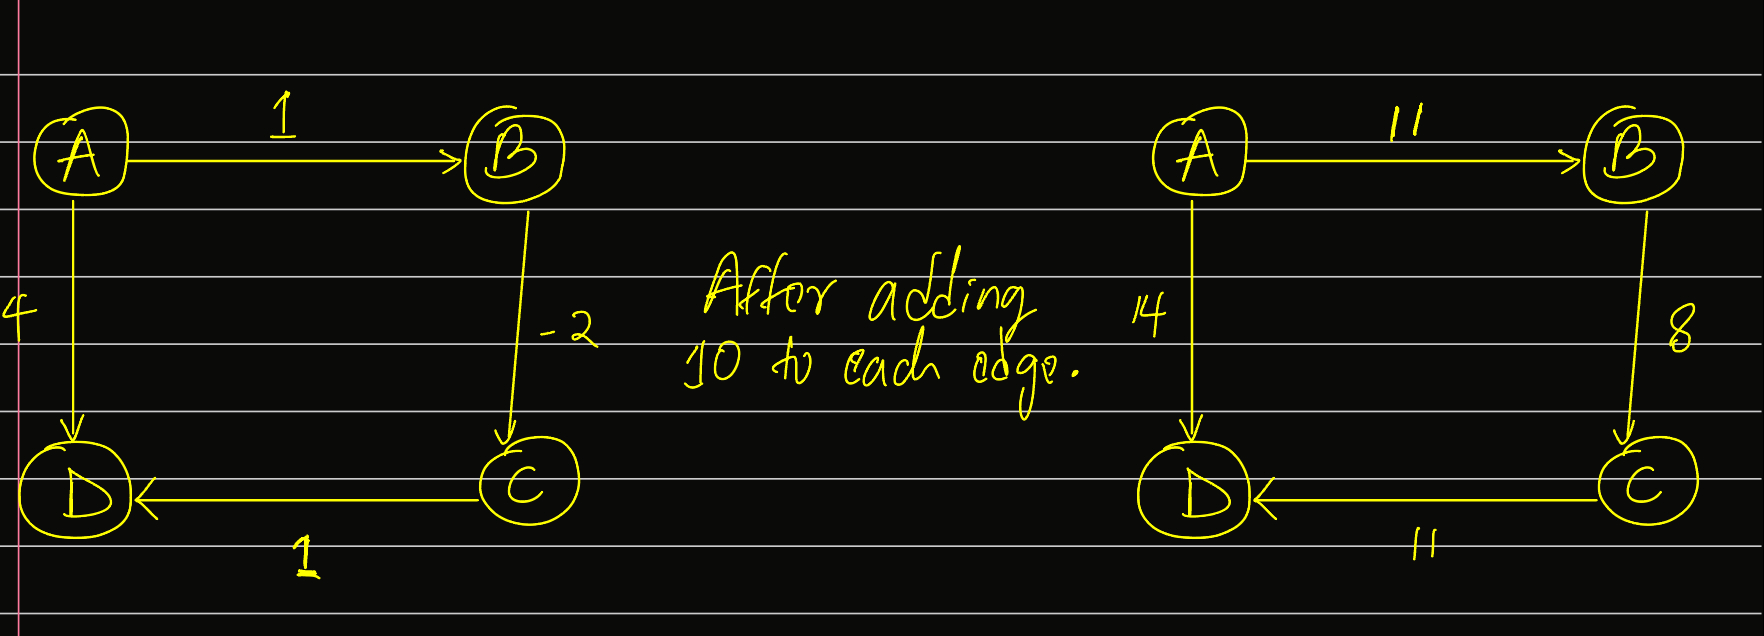
\includegraphics[width=0.7\textwidth]{Question 2 Counterexample.jpg}
    \caption{Question 2 Counterexample.}
    \label{fig:Q2_Counterexample}
\end{figure}

The left part of \ref{fig:Q2_Counterexample} is the original directed graph. The shortest path, say from A to D, is ABCD with a total path weight of $1+(-2)+1=0$. The right part of \ref{fig:Q2_Counterexample} is after we've added a large constant, 10, to all edges in the original directed graph. Notice all edges have positive weights but the shortest path from A to D has changed to just the edge AD which is not the original shortest path. We have found a counterexample to the claim put forth in the question and have thus definitively proven that just adding a large constant to all edges in your directed paths to make them all positive doesn't necessarily preserve the original shortest path.

\item \textbf{[10 points]} Can we do better than Bellman-Ford?

Assume that you are given a graph and a source vertex.  You 
are told that the graph has the
following property: for every vertex $v$, the weights of the edges
along the shortest path from
$s$ to $v$ are strictly increasing.  Describe an efficient algorithm
to solve the single source shortest path problem
for such a graph.  Explain why your algorithm is correct and give the
runtime.

You may assume that 
there are no negative weight cycles, though there may be negative
edge weights.
 
 Since all the edges are strictly increasing, we could sort them first. Then we go over them in order by connecting the next smallest edge first. Once the vertex is already connected, we don't need to check other options as edges since we know it's already the smallest. Once all vertexes are connected we know we are done with the graph. The runtime would be the same as the sorting algorithm which is quick sort and $O(|e|log|e|)$.  
 
 \item \textbf{[10 points]} Suggesting interesting routes

Let $G$ be an undirected graph with $n$ vertices 
(representing major 
attractions) and weighted edges (representing roads and their lengths).  
The {\em boringness} of a path between vertices $u$ and $v$ in $G$ is
defined to be the maximum weight among all edges on that path.  The
{\em cob (coefficient of boringness)} of a pair $(u,v)$ is the
minimum boringness over all paths from $u$ to $v$.

The weights (lengths of the roads between the vertices) are specified
by a symmetric $n \times n$ adjacency matrix where the element in row
$i$ and column $j$ specifies the weight of the edge between vertices
$i$ and $j$ and is $\infty$ if no such edge exists.

\begin{enumerate}

\item Describe a modification to the Floyd-Warshall Algorithm to compute the cobs of all pairs of vertices in the graph and very briefly explain why it is correct.

\textbf{Answer}:
The original Floyd-Warshall Algorithm has the following pseudocode:

\begin{figure}[h]
\centering
    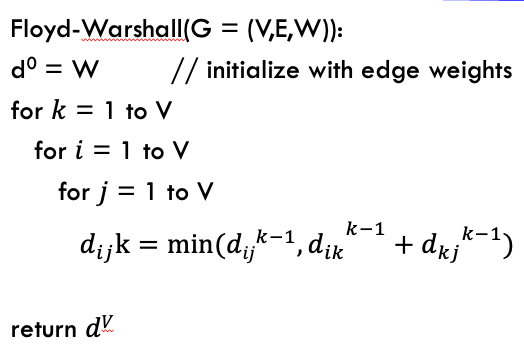
\includegraphics[width=0.5\textwidth]{Floyd-Warshall Algorithm.png}
    \caption{Original Floyd-Warshall Algorithm}
    \label{fig:Floyd-Warshall_Algorithm.}
\end{figure}

Consider the traditional Floyd-Warshall algorithm, as referenced in \ref{fig:Floyd-Warshall_Algorithm.}, which employs dynamic programming to sum the weights along paths, particularly through the combination of $d_{ik}^{k-1}+d_{kj}^{k-1}$. In contrast, in the context of identifying captivating routes, our objective shifts to monitoring the smallest of the largest edge weights encountered during the graph traversal. Consequently, while the overarching framework of the Floyd-Warshall algorithm is preserved, the computation of the cob shifts from the original weight accumulation. Instead, it initially identifies the greater weight between $cob_{ik}^{k-1}$ and $cob_{kj}^{k-1}$, followed by determining the lesser weight across this collected set of maximal weights. The adapted version of the Floyd-Warshall algorithm is therefore:

\begin{figure}[h]
\centering
    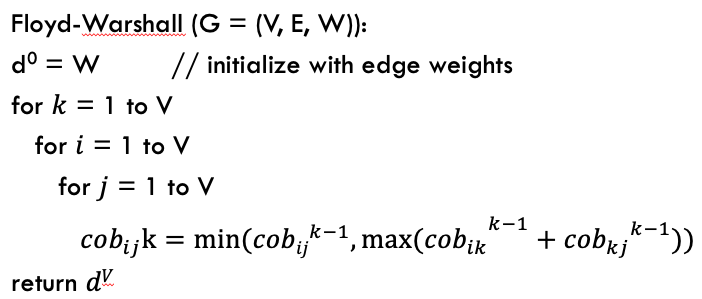
\includegraphics[width=0.5\textwidth]{COB Floyd-Warshall Algorithm.png}
    \caption{COB Floyd-Warshall Algorithm}
    \label{fig:COB Floyd-Warshall_Algorithm.}
\end{figure}

\item What is the running time of your algorithm to compute the cobs?  Explain briefly.

\textbf{Answer}:
The pseudocode still retains much of the core structure of the original Floyd-Warshall algorithm, that is, the 3 nested for-loops thus the runtime of the COB Floyd-Warshall algorithm is similar to the original which is $\Theta(V^3)$.


  
  \end{enumerate}

\item \textbf{[13 points]} Bor\.{u}vka's Algorithm

\vspace*{.2cm}
The first algorithm for computing minimum spanning trees was published 
by the Czech mathematician Otakar Bar\.{u}vka in 1926 and was used for 
laying out electrical networks.  It goes as follows:

\begin{verbatim}
  A = {};  \\ Comment:  A is a subset of a minimum spanning tree

  Consider the n  vertices in the graph as n connected components;
  while A contains fewer than n-1 edges {
     for each connected component C {
        Find the least weight edge (u,v) with one vertex in C and 
          one vertex not in C;
          Indicate that edge (u,v) is "chosen" but do not add it yet to A;
     }
     Add all "chosen" edges to A;
     Compute the new connected components;
  }
  return A \\ Comment:  This is intended to be a MST! 
\end{verbatim}

Notice that
if $C_1$ and $C_2$ are two different connected components before we begin the for loop,
then inside the for loop the algorithm will choose the least weight edge coming out of component $C_1$ and also the least weight edge coming out of $C_2$.  The edge chosen by $C_1$ might join $C_1$ and $C_2$ into a new connected component, but this new connected component will not be discovered until the for loop has ended!  In other words, both $C_1$ and $C_2$ will each get an opportunity to choose the least weight edges coming out of their components.

\begin{enumerate}
  \item \textbf{[2 points]} Give a counterexample that shows that Bor\.{u}vka's Algorithm doesn't work!!
  (You might find it useful to use the fact that some edges in the graph may have the same weight.)
  Show your counterexample graph and explain carefully why Bor\.{u}vka's Algorithm would
 not compute a minimum spanning tree in this case.

\begin{figure}
    \centering
    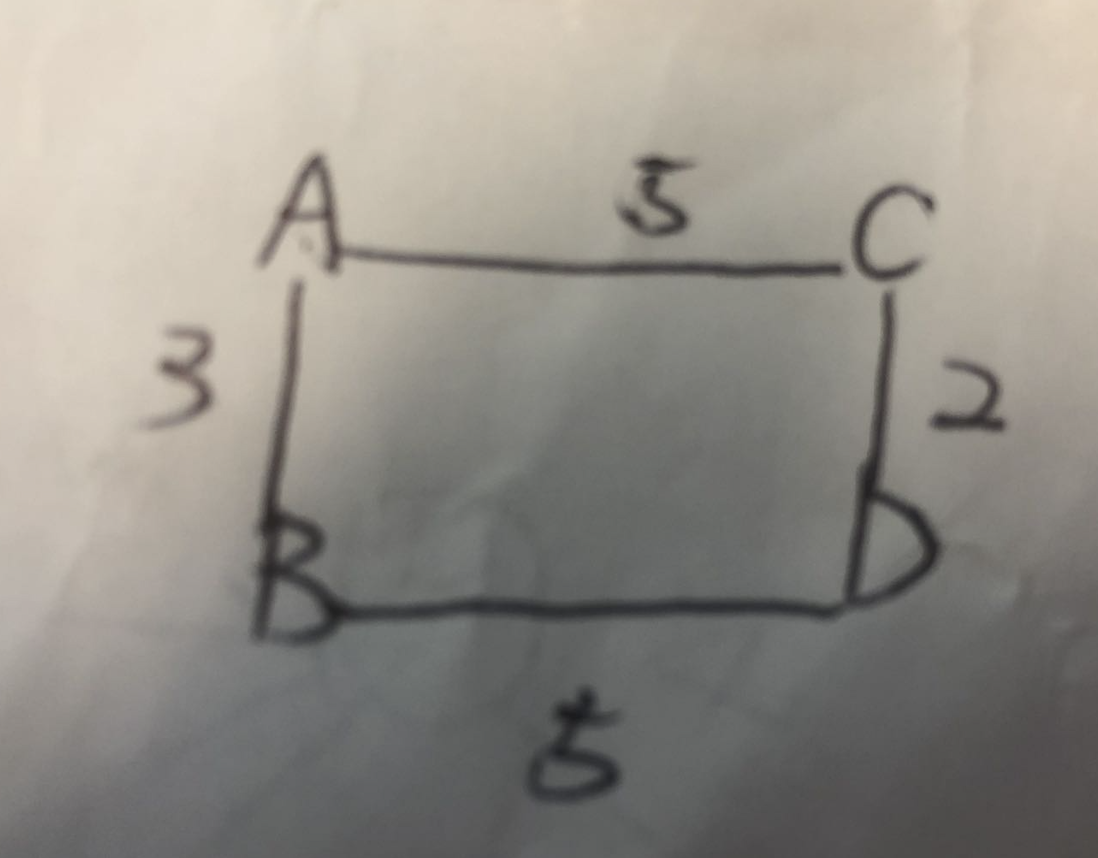
\includegraphics[width=0.5\linewidth]{Sc.png}
    \caption{Enter Caption}
    \label{fig:enter-label}
\end{figure}
In this case the algorithms : from A would pick the minimum edges 3 which connect A to B;   from B would pick the minimum edges 3 which connect B to A; from C would pick the minimum edges 2 which connect C to D; from D would pick the minimum edges 2 which connect D to C; then we quit the for loop and add the edges, therefore after first iteration only A and B and C to D is connected. Since now the graph only has 2 edges is smaller than n-1 =3 edges, we go into the loop again. Now AB is a component and CD is a component, we pick AC which is 5 connecting A and C, but according to the algorithm, since the edge from B to D is also 5 there's a chance the algorithms end up picking that edge as well, in that case we may have A connected to C and B connected to D. In this case, the graph form a rectangle which would not be a MST since it's a cycle and connected unnecessary edges by having both AC and BD connected. 
 \item \textbf{[5 points]}  Now assume that no two edges in the graph have the same weight.  Such a graph has exactly one minimum spanning tree (you may just use this fact here, although you can think about how to prove it!)
Under this assumption, prove that Bor\.{u}vka's Algorithm is correct.

Since there are no two edges have same value, we could consider Bor\.{u}vka's Algorithm doing the same thing as the cut property from the minimum spanning tree. Since all of the edges have different values so there must be only one MST and the cut property says the edge with minimum value in the cut would be in the same MST. . According to this algorithm, we are picking the edges  with the minimum value, which is what the cut property is doing and when we draw a line between two unconnected components and pick the minimum edges and connect them, since we don't have edges sharing the same value, that means we would not connect both of them under the cut property, therefore ensuring we only connect the minimal edges forming the MST.  So everytime we pick the edge with the minimum value from the algorithms, it must be the same edge cutting property picked for the MST

\item \textbf{[3 points]} Why doesn't your proof from part (b) work if some edges in the graph have the same weights?
Because if we have two edges sharing the same value, when going through the part of the algorithms finding the least weight edge (u,v) with one vertex in C and not in C, we may end up confused or connecting all of the edges sharing the same value which may lead to cycle or not forming MST while we may only need to connect one of them. 


\item \textbf{[3 points]} How could Bor\.{u}vka's Algorithm be modified slightly to work in the most general case
that edge weights are not necessarily distinct?  Explain briefly why this modification preserves the correctness of the algorithm.
If two edges share the same value, we could let the algorithm distinguish two edges from their vertices. So if  two edges have the same value, the algorithm can prioritize the edge by the lexicographical order of the vertices' labels. By doing so we could avoid connecting multiple edges sharing the same value as in part (a) while we only need to connect one. 

\end{enumerate}
\end{enumerate}

\end{document}
